\documentclass{standalone}
\usepackage{tikz}
\usetikzlibrary{patterns, positioning}


\begin{document}
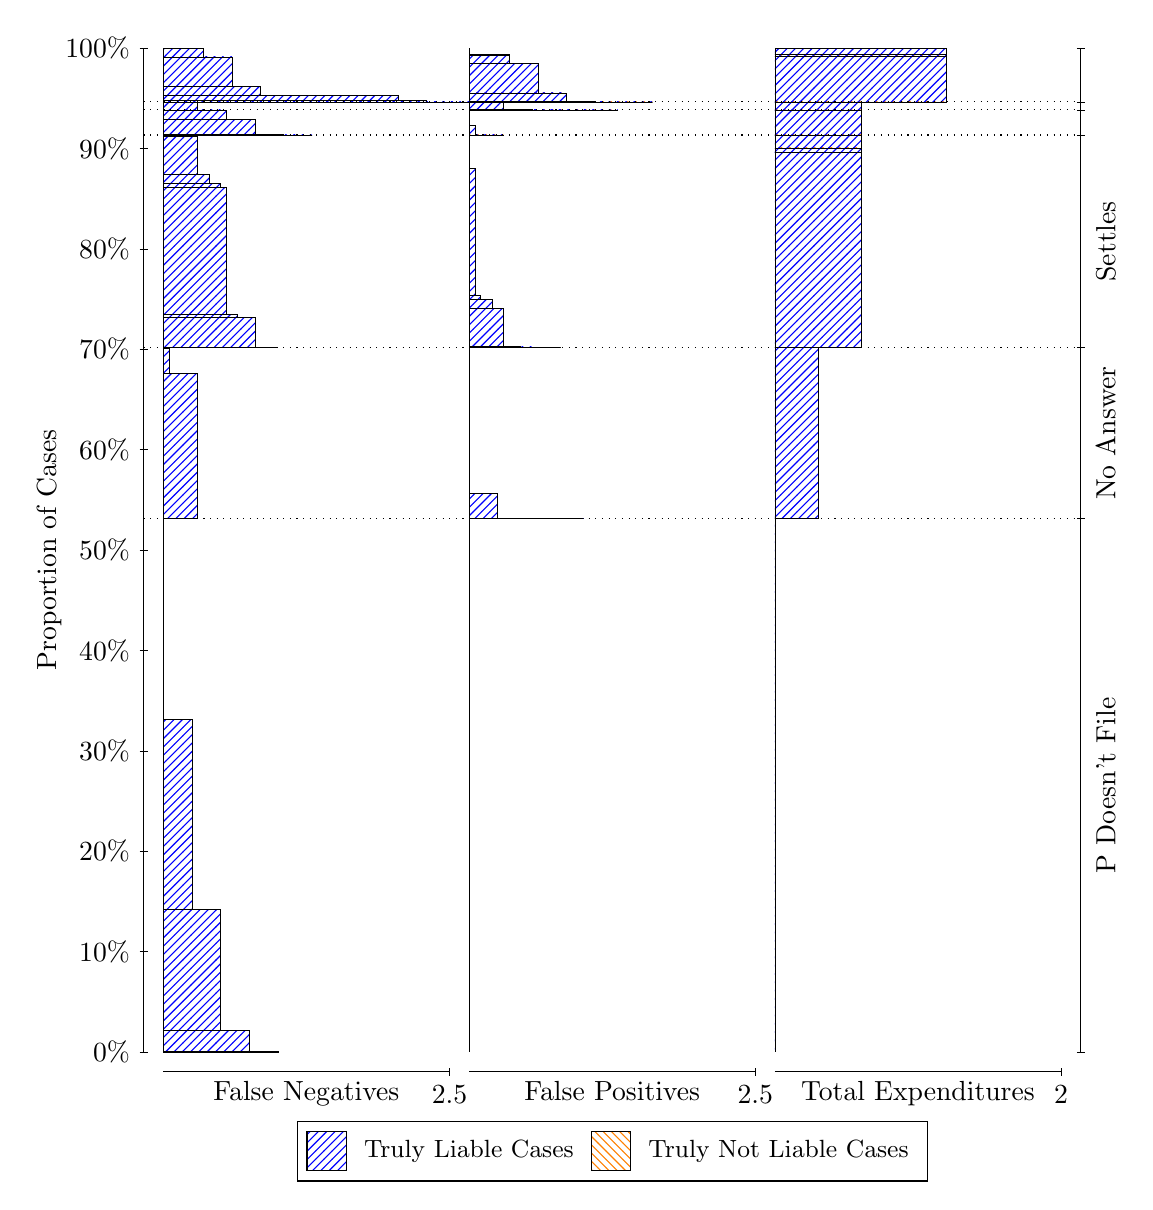
\begin{tikzpicture}
\draw[black, very thin] (1.5,1.75) -- (1.5,14.5);
\node[rotate=90, text=black, anchor=center] at (0.3, 8.125) {Proportion of Cases};
\draw[black, very thin] (1.45,1.75) -- (1.55,1.75);
\node[text=black, anchor=east] at (1.45, 1.75) {0\%};
\draw[black, very thin] (1.45,3.025) -- (1.55,3.025);
\node[text=black, anchor=east] at (1.45, 3.025) {10\%};
\draw[black, very thin] (1.45,4.3) -- (1.55,4.3);
\node[text=black, anchor=east] at (1.45, 4.3) {20\%};
\draw[black, very thin] (1.45,5.575) -- (1.55,5.575);
\node[text=black, anchor=east] at (1.45, 5.575) {30\%};
\draw[black, very thin] (1.45,6.85) -- (1.55,6.85);
\node[text=black, anchor=east] at (1.45, 6.85) {40\%};
\draw[black, very thin] (1.45,8.125) -- (1.55,8.125);
\node[text=black, anchor=east] at (1.45, 8.125) {50\%};
\draw[black, very thin] (1.45,9.4) -- (1.55,9.4);
\node[text=black, anchor=east] at (1.45, 9.4) {60\%};
\draw[black, very thin] (1.45,10.675) -- (1.55,10.675);
\node[text=black, anchor=east] at (1.45, 10.675) {70\%};
\draw[black, very thin] (1.45,11.95) -- (1.55,11.95);
\node[text=black, anchor=east] at (1.45, 11.95) {80\%};
\draw[black, very thin] (1.45,13.225) -- (1.55,13.225);
\node[text=black, anchor=east] at (1.45, 13.225) {90\%};
\draw[black, very thin] (1.45,14.5) -- (1.55,14.5);
\node[text=black, anchor=east] at (1.45, 14.5) {100\%};

\draw[black, very thin] (13.4,1.75) -- (13.4,14.5);
\draw[black, very thin] (13.35,1.75) -- (13.45,1.75);
\node[anchor=west] at (13.35, 1.75) {};
\draw[black, very thin] (13.35,8.5224) -- (13.45,8.5224);
\node[anchor=west] at (13.35, 8.5224) {};
\draw[black, very thin] (13.35,10.694) -- (13.45,10.694);
\node[anchor=west] at (13.35, 10.694) {};
\draw[black, very thin] (13.35,13.396) -- (13.45,13.396);
\node[anchor=west] at (13.35, 13.396) {};
\draw[black, very thin] (13.35,13.714) -- (13.45,13.714);
\node[anchor=west] at (13.35, 13.714) {};
\draw[black, very thin] (13.35,13.817) -- (13.45,13.817);
\node[anchor=west] at (13.35, 13.817) {};
\draw[black, very thin] (13.35,14.5) -- (13.45,14.5);
\node[anchor=west] at (13.35, 14.5) {};

\draw[black, very thin, pattern color=blue, pattern=north east lines] (1.75,1.75) rectangle (3.2033,1.7527);
\draw[black, very thin, pattern color=blue, pattern=north east lines] (1.75,1.7527) rectangle (2.84,2.0195);
\draw[black, very thin, pattern color=blue, pattern=north east lines] (1.75,2.0195) rectangle (2.4767,3.5655);
\draw[black, very thin, pattern color=blue, pattern=north east lines] (1.75,3.5655) rectangle (2.1133,5.9738);
\draw[black, very thin, pattern color=orange, pattern=north west lines] (1.75,5.9738) rectangle (1.75,5.9738);
\draw[black, very thin, pattern color=blue, pattern=north east lines] (1.75,5.9738) rectangle (1.75,8.5224);
\draw[black, very thin, pattern color=blue, pattern=north east lines] (1.75,8.5224) rectangle (2.186,10.371);
\draw[black, very thin, pattern color=blue, pattern=north east lines] (1.75,10.371) rectangle (1.8227,10.693);
\draw[black, very thin, pattern color=orange, pattern=north west lines] (1.75,10.693) rectangle (1.75,10.693);
\draw[black, very thin, pattern color=blue, pattern=north east lines] (1.75,10.693) rectangle (1.75,10.694);
\draw[black, very thin, pattern color=blue, pattern=north east lines] (1.75,10.694) rectangle (3.2033,10.694);
\draw[black, very thin, pattern color=blue, pattern=north east lines] (1.75,10.694) rectangle (3.058,10.694);
\draw[black, very thin, pattern color=blue, pattern=north east lines] (1.75,10.694) rectangle (2.9127,11.075);
\draw[black, very thin, pattern color=blue, pattern=north east lines] (1.75,11.075) rectangle (2.84,11.077);
\draw[black, very thin, pattern color=blue, pattern=north east lines] (1.75,11.077) rectangle (2.6947,11.115);
\draw[black, very thin, pattern color=blue, pattern=north east lines] (1.75,11.115) rectangle (2.5493,12.729);
\draw[black, very thin, pattern color=blue, pattern=north east lines] (1.75,12.729) rectangle (2.4767,12.778);
\draw[black, very thin, pattern color=blue, pattern=north east lines] (1.75,12.778) rectangle (2.3313,12.899);
\draw[black, very thin, pattern color=blue, pattern=north east lines] (1.75,12.899) rectangle (2.186,13.378);
\draw[black, very thin, pattern color=blue, pattern=north east lines] (1.75,13.378) rectangle (2.1133,13.381);
\draw[black, very thin, pattern color=blue, pattern=north east lines] (1.75,13.381) rectangle (1.968,13.386);
\draw[black, very thin, pattern color=blue, pattern=north east lines] (1.75,13.386) rectangle (1.8227,13.396);
\draw[black, very thin, pattern color=orange, pattern=north west lines] (1.75,13.396) rectangle (1.75,13.396);
\draw[black, very thin, pattern color=blue, pattern=north east lines] (1.75,13.396) rectangle (1.75,13.396);
\draw[black, very thin, pattern color=blue, pattern=north east lines] (1.75,13.396) rectangle (3.6393,13.396);
\draw[black, very thin, pattern color=blue, pattern=north east lines] (1.75,13.396) rectangle (3.276,13.401);
\draw[black, very thin, pattern color=blue, pattern=north east lines] (1.75,13.401) rectangle (2.9127,13.592);
\draw[black, very thin, pattern color=blue, pattern=north east lines] (1.75,13.592) rectangle (2.5493,13.713);
\draw[black, very thin, pattern color=blue, pattern=north east lines] (1.75,13.713) rectangle (2.186,13.714);
\draw[black, very thin, pattern color=orange, pattern=north west lines] (1.75,13.714) rectangle (1.75,13.714);
\draw[black, very thin, pattern color=blue, pattern=north east lines] (1.75,13.714) rectangle (2.186,13.813);
\draw[black, very thin, pattern color=blue, pattern=north east lines] (1.75,13.813) rectangle (1.8227,13.817);
\draw[black, very thin, pattern color=orange, pattern=north west lines] (1.75,13.817) rectangle (1.75,13.817);
\draw[black, very thin, pattern color=blue, pattern=north east lines] (1.75,13.817) rectangle (1.75,13.817);
\draw[black, very thin, pattern color=blue, pattern=north east lines] (1.75,13.817) rectangle (5.8193,13.817);
\draw[black, very thin, pattern color=blue, pattern=north east lines] (1.75,13.817) rectangle (5.456,13.817);
\draw[black, very thin, pattern color=blue, pattern=north east lines] (1.75,13.817) rectangle (5.0927,13.834);
\draw[black, very thin, pattern color=blue, pattern=north east lines] (1.75,13.834) rectangle (4.7293,13.899);
\draw[black, very thin, pattern color=blue, pattern=north east lines] (1.75,13.899) rectangle (4.366,13.9);
\draw[black, very thin, pattern color=blue, pattern=north east lines] (1.75,13.9) rectangle (4.0027,13.9);
\draw[black, very thin, pattern color=blue, pattern=north east lines] (1.75,13.9) rectangle (3.712,13.9);
\draw[black, very thin, pattern color=blue, pattern=north east lines] (1.75,13.9) rectangle (3.6393,13.9);
\draw[black, very thin, pattern color=blue, pattern=north east lines] (1.75,13.9) rectangle (3.3487,13.9);
\draw[black, very thin, pattern color=blue, pattern=north east lines] (1.75,13.9) rectangle (2.9853,14.011);
\draw[black, very thin, pattern color=blue, pattern=north east lines] (1.75,14.011) rectangle (2.622,14.388);
\draw[black, very thin, pattern color=blue, pattern=north east lines] (1.75,14.388) rectangle (2.2587,14.496);
\draw[black, very thin, pattern color=blue, pattern=north east lines] (1.75,14.496) rectangle (1.8953,14.5);
\draw[black, very thin, pattern color=orange, pattern=north west lines] (1.75,14.5) rectangle (1.75,14.5);
\draw[black, very thin, pattern color=blue, pattern=north east lines] (1.75,14.5) rectangle (1.75,14.5);
\draw[black, very thin, pattern color=orange, pattern=north west lines] (5.6333,1.75) rectangle (5.6333,1.75);
\draw[black, very thin, pattern color=blue, pattern=north east lines] (5.6333,1.75) rectangle (5.6333,8.5224);
\draw[black, very thin, pattern color=orange, pattern=north west lines] (5.6333,8.5224) rectangle (7.0867,8.5224);
\draw[black, very thin, pattern color=blue, pattern=north east lines] (5.6333,8.5224) rectangle (7.0867,8.5224);
\draw[black, very thin, pattern color=blue, pattern=north east lines] (5.6333,8.5224) rectangle (6.7233,8.5224);
\draw[black, very thin, pattern color=blue, pattern=north east lines] (5.6333,8.5224) rectangle (6.36,8.5236);
\draw[black, very thin, pattern color=blue, pattern=north east lines] (5.6333,8.5236) rectangle (5.9967,8.8452);
\draw[black, very thin, pattern color=blue, pattern=north east lines] (5.6333,8.8452) rectangle (5.6333,10.694);
\draw[black, very thin, pattern color=orange, pattern=north west lines] (5.6333,10.694) rectangle (6.796,10.694);
\draw[black, very thin, pattern color=blue, pattern=north east lines] (5.6333,10.694) rectangle (6.796,10.694);
\draw[black, very thin, pattern color=orange, pattern=north west lines] (5.6333,10.694) rectangle (6.6507,10.694);
\draw[black, very thin, pattern color=blue, pattern=north east lines] (5.6333,10.694) rectangle (6.6507,10.694);
\draw[black, very thin, pattern color=orange, pattern=north west lines] (5.6333,10.694) rectangle (6.5053,10.694);
\draw[black, very thin, pattern color=blue, pattern=north east lines] (5.6333,10.694) rectangle (6.5053,10.694);
\draw[black, very thin, pattern color=blue, pattern=north east lines] (5.6333,10.694) rectangle (6.4327,10.704);
\draw[black, very thin, pattern color=blue, pattern=north east lines] (5.6333,10.704) rectangle (6.2873,10.708);
\draw[black, very thin, pattern color=blue, pattern=north east lines] (5.6333,10.708) rectangle (6.142,10.711);
\draw[black, very thin, pattern color=blue, pattern=north east lines] (5.6333,10.711) rectangle (6.0693,11.191);
\draw[black, very thin, pattern color=blue, pattern=north east lines] (5.6333,11.191) rectangle (5.924,11.312);
\draw[black, very thin, pattern color=blue, pattern=north east lines] (5.6333,11.312) rectangle (5.7787,11.361);
\draw[black, very thin, pattern color=blue, pattern=north east lines] (5.6333,11.361) rectangle (5.706,12.975);
\draw[black, very thin, pattern color=blue, pattern=north east lines] (5.6333,12.975) rectangle (5.6333,13.396);
\draw[black, very thin, pattern color=orange, pattern=north west lines] (5.6333,13.396) rectangle (6.0693,13.396);
\draw[black, very thin, pattern color=blue, pattern=north east lines] (5.6333,13.396) rectangle (6.0693,13.397);
\draw[black, very thin, pattern color=blue, pattern=north east lines] (5.6333,13.397) rectangle (5.706,13.518);
\draw[black, very thin, pattern color=blue, pattern=north east lines] (5.6333,13.518) rectangle (5.6333,13.714);
\draw[black, very thin, pattern color=orange, pattern=north west lines] (5.6333,13.714) rectangle (7.5227,13.714);
\draw[black, very thin, pattern color=blue, pattern=north east lines] (5.6333,13.714) rectangle (7.5227,13.714);
\draw[black, very thin, pattern color=blue, pattern=north east lines] (5.6333,13.714) rectangle (7.1593,13.714);
\draw[black, very thin, pattern color=blue, pattern=north east lines] (5.6333,13.714) rectangle (6.796,13.714);
\draw[black, very thin, pattern color=blue, pattern=north east lines] (5.6333,13.714) rectangle (6.4327,13.718);
\draw[black, very thin, pattern color=blue, pattern=north east lines] (5.6333,13.718) rectangle (6.0693,13.817);
\draw[black, very thin, pattern color=orange, pattern=north west lines] (5.6333,13.817) rectangle (7.9587,13.817);
\draw[black, very thin, pattern color=blue, pattern=north east lines] (5.6333,13.817) rectangle (7.9587,13.817);
\draw[black, very thin, pattern color=orange, pattern=north west lines] (5.6333,13.817) rectangle (7.5953,13.817);
\draw[black, very thin, pattern color=blue, pattern=north east lines] (5.6333,13.817) rectangle (7.5953,13.817);
\draw[black, very thin, pattern color=orange, pattern=north west lines] (5.6333,13.817) rectangle (7.232,13.817);
\draw[black, very thin, pattern color=blue, pattern=north east lines] (5.6333,13.817) rectangle (7.232,13.821);
\draw[black, very thin, pattern color=blue, pattern=north east lines] (5.6333,13.821) rectangle (6.8687,13.929);
\draw[black, very thin, pattern color=orange, pattern=north west lines] (5.6333,13.929) rectangle (6.8687,13.929);
\draw[black, very thin, pattern color=blue, pattern=north east lines] (5.6333,13.929) rectangle (6.8687,13.929);
\draw[black, very thin, pattern color=blue, pattern=north east lines] (5.6333,13.929) rectangle (6.5053,14.305);
\draw[black, very thin, pattern color=blue, pattern=north east lines] (5.6333,14.305) rectangle (6.5053,14.307);
\draw[black, very thin, pattern color=blue, pattern=north east lines] (5.6333,14.307) rectangle (6.142,14.403);
\draw[black, very thin, pattern color=blue, pattern=north east lines] (5.6333,14.403) rectangle (6.142,14.417);
\draw[black, very thin, pattern color=blue, pattern=north east lines] (5.6333,14.417) rectangle (5.7787,14.417);
\draw[black, very thin, pattern color=blue, pattern=north east lines] (5.6333,14.417) rectangle (5.7787,14.417);
\draw[black, very thin, pattern color=orange, pattern=north west lines] (5.6333,14.417) rectangle (5.6333,14.417);
\draw[black, very thin, pattern color=blue, pattern=north east lines] (5.6333,14.417) rectangle (5.6333,14.5);
\draw[black, very thin, pattern color=orange, pattern=north west lines] (9.5167,1.75) rectangle (9.5167,1.75);
\draw[black, very thin, pattern color=blue, pattern=north east lines] (9.5167,1.75) rectangle (9.5167,8.5224);
\draw[black, very thin, pattern color=orange, pattern=north west lines] (9.5167,8.5224) rectangle (10.062,8.5224);
\draw[black, very thin, pattern color=blue, pattern=north east lines] (9.5167,8.5224) rectangle (10.062,10.694);
\draw[black, very thin, pattern color=orange, pattern=north west lines] (9.5167,10.694) rectangle (10.607,10.694);
\draw[black, very thin, pattern color=blue, pattern=north east lines] (9.5167,10.694) rectangle (10.607,13.179);
\draw[black, very thin, pattern color=orange, pattern=north west lines] (9.5167,13.179) rectangle (10.607,13.179);
\draw[black, very thin, pattern color=blue, pattern=north east lines] (9.5167,13.179) rectangle (10.607,13.233);
\draw[black, very thin, pattern color=orange, pattern=north west lines] (9.5167,13.233) rectangle (10.607,13.233);
\draw[black, very thin, pattern color=blue, pattern=north east lines] (9.5167,13.233) rectangle (10.607,13.396);
\draw[black, very thin, pattern color=orange, pattern=north west lines] (9.5167,13.396) rectangle (10.607,13.396);
\draw[black, very thin, pattern color=blue, pattern=north east lines] (9.5167,13.396) rectangle (10.607,13.714);
\draw[black, very thin, pattern color=orange, pattern=north west lines] (9.5167,13.714) rectangle (10.607,13.714);
\draw[black, very thin, pattern color=blue, pattern=north east lines] (9.5167,13.714) rectangle (10.607,13.817);
\draw[black, very thin, pattern color=orange, pattern=north west lines] (9.5167,13.817) rectangle (11.697,13.817);
\draw[black, very thin, pattern color=blue, pattern=north east lines] (9.5167,13.817) rectangle (11.697,14.401);
\draw[black, very thin, pattern color=orange, pattern=north west lines] (9.5167,14.401) rectangle (11.697,14.401);
\draw[black, very thin, pattern color=blue, pattern=north east lines] (9.5167,14.401) rectangle (11.697,14.417);
\draw[black, very thin, pattern color=orange, pattern=north west lines] (9.5167,14.417) rectangle (11.697,14.417);
\draw[black, very thin, pattern color=blue, pattern=north east lines] (9.5167,14.417) rectangle (11.697,14.5);
\draw[black, dotted] (1.5,8.5224) -- (13.4,8.5224);
\draw[black, dotted] (1.5,10.694) -- (13.4,10.694);
\draw[black, dotted] (1.5,13.396) -- (13.4,13.396);
\draw[black, dotted] (1.5,13.714) -- (13.4,13.714);
\draw[black, dotted] (1.5,13.817) -- (13.4,13.817);
\draw[black, very thin] (1.75,1.5) -- (5.3833,1.5);
\node[text=black, anchor=north] at (3.5667, 1.5) {False Negatives};
\draw[black, very thin] (5.3833,1.45) -- (5.3833,1.55);
\node[text=black, anchor=north] at (5.3833, 1.45) {2.5};

\draw[black, very thin] (5.6333,1.5) -- (9.2667,1.5);
\node[text=black, anchor=north] at (7.45, 1.5) {False Positives};
\draw[black, very thin] (9.2667,1.45) -- (9.2667,1.55);
\node[text=black, anchor=north] at (9.2667, 1.45) {2.5};

\draw[black, very thin] (9.5167,1.5) -- (13.15,1.5);
\node[text=black, anchor=north] at (11.333, 1.5) {Total Expenditures};
\draw[black, very thin] (13.15,1.45) -- (13.15,1.55);
\node[text=black, anchor=north] at (13.15, 1.45) {2};

\node[text=black, centered, rotate=90] at (13.72, 5.1362) {P Doesn't File};
\node[text=black, centered, rotate=90] at (13.72, 9.6081) {No Answer};
\node[text=black, centered, rotate=90] at (13.72, 12.045) {Settles};




\draw (7.449999999999999,1.5) node[draw=none] (baseCoordinate) {};
\begin{scope}[align=center]
        \matrix[scale=0.5, draw=black, below=0.5cm of baseCoordinate, nodes={draw}, column sep=0.1cm]{
            \node[rectangle, draw, minimum width=0.5cm, minimum height=0.5cm, pattern color=blue, pattern=north east lines] {}; &
            \node[draw=none, font=\small, text=black] (B) {Truly Liable Cases}; &
            \node[rectangle, draw, minimum width=0.5cm, minimum height=0.5cm, pattern color=orange, pattern=north west lines] {}; &
            \node[draw=none, font=\small, text=black] (B) {Truly Not Liable Cases}; \\
            };
\end{scope}

\end{tikzpicture}
\end{document}